\section{Measurement Setups}
To experimentally validate the design, a set of measurements was carried out covering small-signal behavior, large-signal power performance, and nonlinear characterization. Each measurement required a dedicated setup, described in the following subsections.

% =========================================================================== %
\subsection{S-Parameters Measurement Setup}
S-parameters were measured to validate the matching network design and characterize the small-signal behavior of the amplifier. A Keysight N5242B PNA-X vector network analyzer (VNA), calibrated using the TOSM method with a Keysight 85052B calibration kit, was employed. A fixed 30\,dB attenuator was inserted at the output port to protect the VNA receiver from high power levels. Consequently, only $S_{21}$ and $S_{11}$ are reported. The attenuator's effect was de-embedded from the measured $S_{21}$ by adding the nominal attenuator value.

% =========================================================================== %
\subsection{Power Output Measurement Setup}
A power output measurement was carried out to characterize the large-signal behavior of the amplifier. Since the device under test requires drive levels beyond the native output capability of the measurement instrument, a Mini-Circuits ZX60-83LN12+ driver amplifier was inserted between the Keysight N5242B signal source and the PA under test. Output power was measured with a Keysight U8485A power sensor preceded by a 20\,dB attenuator and a 10\,dB attenuator, as shown in Fig.~\ref{fig:power_meas_setup}. The input was swept in 2.5\,dBm steps at the nominal operating frequency of 2.2\,GHz. The values obtained from this measurement were used to determine the gain and the 1\,dB compression point of the amplifier.

\begin{figure}[b]
    \centering
    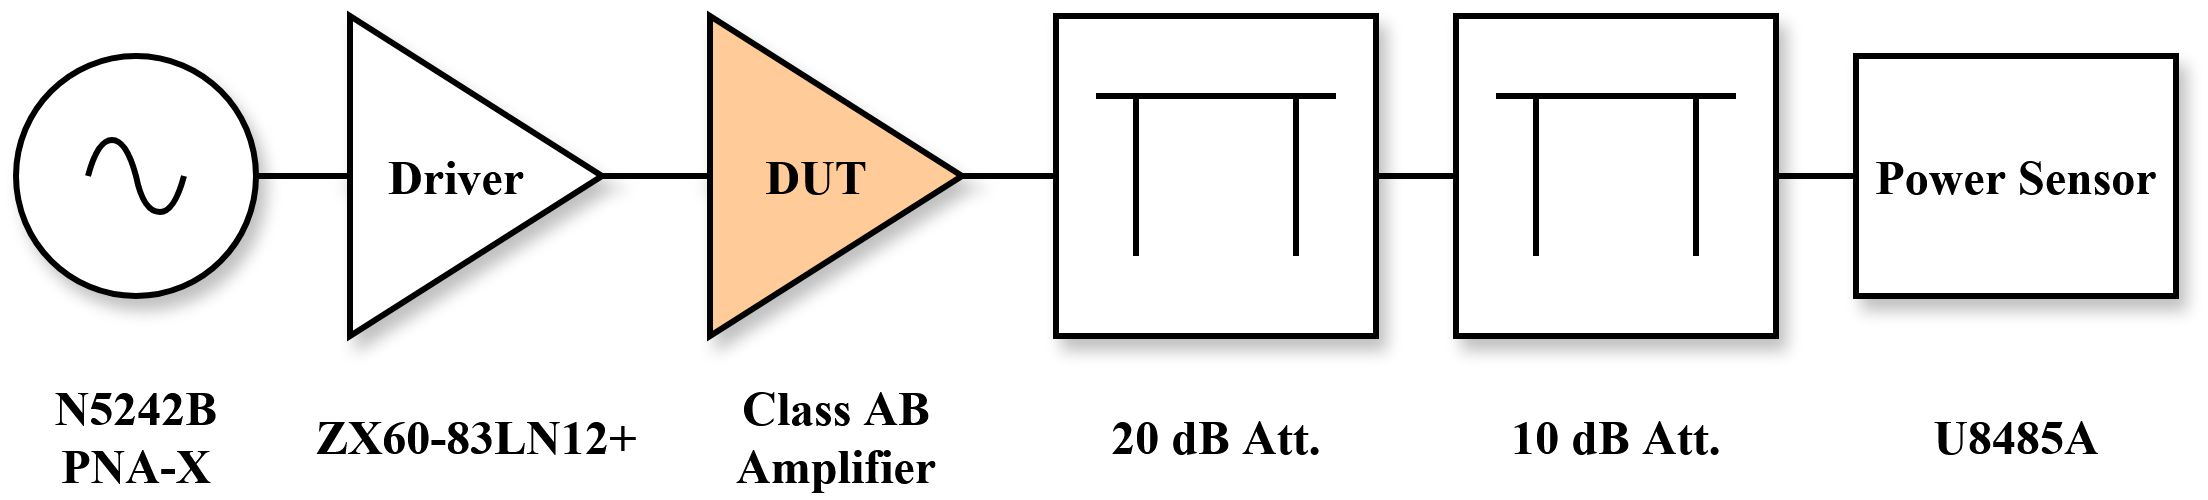
\includegraphics[width=0.48\textwidth]{imgs/p1db_blocks.png}
    \caption{Output power measurement setup including the PNA as RF signal source, driver amplifier, DUT, two cascaded attenuators at the DUT output, and a power sensor.}
    \label{fig:power_meas_setup}
\end{figure}

% =========================================================================== %
\subsection{Harmonic Power Measurement Setup}
Due to the intrinsic nonlinearity of any active device, as well as the operating class at which the amplifier is biased, PAs generate harmonic distortion that degrades spectral purity and may cause out-of-band interference. To characterize this behavior, the second and third harmonics were measured using a Siglent SSG3032X-IQE signal generator as the CW RF source at 2.2\,GHz and a Keysight N9322C spectrum analyzer at the output, as illustrated in Fig.~\ref{fig:hb_setup}. A 20\,dB attenuator was placed at the analyzer input for protection. The input power was swept from 0\,dBm to 20\,dBm in 5\,dBm steps.

\begin{figure}[t]
    \centering
    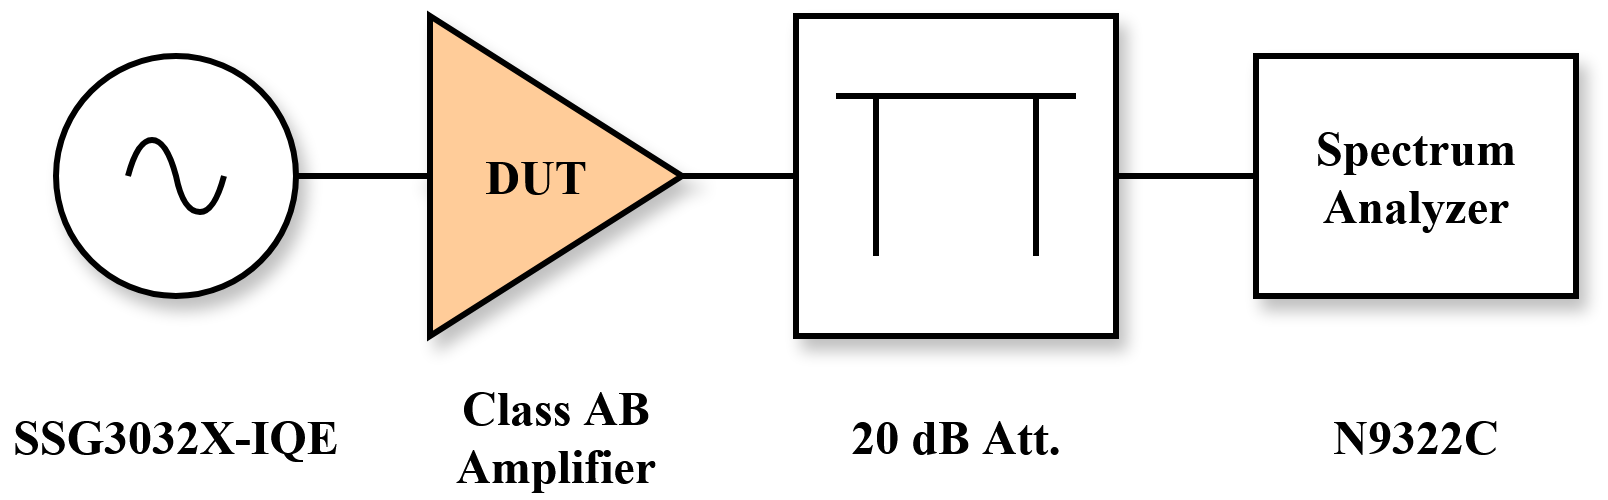
\includegraphics[width=0.48\textwidth]{imgs/harmonic_balance_blocks.png}
    \caption{Harmonic power measurement setup including the RF signal source, DUT, the 20 dB attenuator, and the spectrum analyzer.}
    \label{fig:hb_setup}
\end{figure}

% =========================================================================== %
\subsection{OIP3 Measurement Setup}
The third-order intercept point (OIP3) was obtained using the "IMD Sweep"(S93087B IMD) software application of the Keysight N5242B PNA-X VNA \cite{KeysightPNAConfig}. As with the power output measurement, a Mini-Circuits ZX60-83LN12+ driver amplifier was added between the VNA's signal source and the DUT to reach the drive levels required to manifest the amplifier's nonlinear effects. Also, two attenuators of 20\,dB and 10\,dB were added to the DUT output to protect the VNA ports.

The frequency separation of the tones was set to 10 MHz, and their power was set to $P_{in} = -5 \,\text{dBm}$ 
